\section{Mengen und Funktionen}

\begin{frame}
  {Was ist eine Menge?}
  \onslide<+->
  \onslide<+->
  Eine \alert{frei definierbare ungeordnete Sammlung von diskreten Objekten}\\
  \begin{itemize}[<+->]
    \item Zahlen
    \item Menschen
    \item Schuhe
    \item Wörter
    \item \ldots
      \Halbzeile
    \item nicht unbedingt zweckgebunden
    \item \orongsch{jedes Objekt maximal einmal in jeder Menge}
  \end{itemize}
  \centering
  \Zeile
  \onslide<+->
  Das Wesentliche von heute in \citet[Kapitel~1--4]{ParteeEa1990}
\end{frame}

\begin{frame}
  {Notation und Beispiele für Mengen}
  \onslide<+->
  \onslide<+->
  Mengendefinition \alert{\{\}}, Elementstatus $\in$\\
  \Zeile
  \begin{itemize}[<+->]
    \item M\Sub{1} = \alert{$\{a,b,c\}$} (Menge von Buchstaben)
      \Halbzeile
    \item N\Sub{1} = \alert{$\{$`my book'$\}$} (einelementige Menge, enthält eine NP)
      \begin{itemize}[<+->]
        \item vs. \alert{N\Sub{2} = $\{$my book$\}$} (einelementige Menge, enthält mein Buch)
        \item vs. \alert{N\Sub{3} = $\{$`my', `book'$\}$} (Menge von Wörtern)
      \end{itemize}
      \Halbzeile
    \item möglich, aber ungewöhnlich: \orongsch{N\Sub{4} = $\{$`my', book$\}$}
      \Halbzeile
    \item definiert über eine Eigenschaft der Elemente (zwei Notationen):\\
      M\Sub{2} = \gruen{$\{$x: x is one of the first three letters of the alphabet$\}$}\\
      M\Sub{2} = \gruen{$\{$x$\|$ x is one of the first three letters of the alphabet$\}$}
      \Halbzeile
    \item \alert{U}: die universelle Menge (alle Objekte)
  \end{itemize}
\end{frame}

\begin{frame}
  {Identität von Mengen}
  \onslide<+->
  \onslide<+->
  Zwei Mengen mit exakt den gleichen Elementen sind \alert{identisch}.\\
  \Zeile 
  \begin{itemize}[<+->]
    \item \alert{\{a, b, c\}} = \gruen{\{x: x is one of the first tree letter of the alphabet\}}
      \Halbzeile
    \item \alert{\{x: x is human\}} = \gruen{\{x: x is from the Earth, a primate but not an ape\}}
  \end{itemize}
\end{frame}

\begin{frame}
  {Teilmengen und Obermengen}
  \onslide<+->
  \onslide<+->
  \alert{Teilmenge} | Eine Menge N, die kein Element enthält,\\
  das nicht auch in Menge M enthalten ist (umg.\ \alert{Obermenge}).\\
  \Halbzeile
  \onslide<+->
  Teilmenge oder Identität $\subseteq$\\
  Obermenge oder Identität $\supseteq$\\
  \Zeile
  \begin{itemize}[<+->]
    \item \{a\} \alert{$\subseteq$} \{a,b,c\} und \{a,b,c\} \alert{$\supseteq$} \{a\}
    \item \{a\} \alert{$\subseteq$} \{a,b,c\} und \{a,b,c\} \alert{$\supseteq$} \{a\} 
    \item \{a,b,c\} \alert{$\subseteq$} \{a,b,c\}
      \Halbzeile
    \item \{a,b,c,d\} \orongsch{$\not\subseteq$} \{a,b,c\} und \{a,b,c\} \orongsch{$\not\supseteq$} \{a,b,c,d\}
      \Halbzeile
    \item \{x: x is human\} \gruen{$\subseteq$} \{x: is an ape\}
  \end{itemize}
\end{frame}


\begin{frame}
  {Echte Teilmengen und Obermengen}
  \onslide<+->
  \onslide<+->
  \alert{Echte Teilmenge} | Eine Menge N, die kein Element enthält,\\
  das nicht auch in Menge M enthalten ist, und die nicht mit M identisch ist.\\
  \Halbzeile
  \onslide<+->
  Echte Teilmenge $\subset$\\
  Echte Obermenge $\supset$\\
  \Zeile
  \begin{itemize}[<+->]
    \item $\{a\}\gruen{\subset}\{a,b,c\}$ und $\{a\}\alert{\subset}\{a,b,c\}$
    \item $\{a,b,c\}\orongsch{\not\subset}\{a,b,c\}$ aber $\{a,b,c\}\orongsch{\subseteq}\{a,b,c\}$
  \end{itemize}
\end{frame}

\begin{frame}
  {Elemente vs.\ Teilmengen}
  \onslide<+->
  \begin{itemize}[<+->]
    \item Achtung bei Mengen von Mengen
      \begin{itemize}[<+->]
        \item \{\{a\}\} \orongsch{$\not\subset$} \{a,b,c\}
        \item \{\{a\}\} \orongsch{$\not\subseteq$} \{a,b,c\}
        \item \{\{a\}\} \orongsch{$\not\in$} \{a,b,c\}
      \end{itemize}
    \Zeile
    \item für leere Menge \grau{\{\} oder $\emptyset$}
      \begin{itemize}[<+->]
        \item \{\} \alert{$\subset$} jede anderen Menge
        \item \{\} \orongsch{$\not\in$} \{\}
      \end{itemize}
  \end{itemize}
\end{frame}

\begin{frame}
  {Logik mit Mengen, Teilmengen und Elementen}
  \onslide<+->
  \begin{itemize}[<+->]
    \item Logik mit Mengen
        \begin{itemize}[<+->]
        \item \textit{Alle Anglistikprofessoren sind menschlich.}\\
          \textit{Herr Webelhuth ist Anglistikprofessor.}
        \item w = Herr Webelhuth\\
          E = \{x: x is professors of English Linguistics\}\\
          H = \{x: x is human\}
        \item Aus \alert{$w\in E$} und \alert{$E\subset H$} folgt \gruen{$w\in H$}
      \end{itemize}
      \Halbzeile
    \item Aber
      \begin{itemize}[<+->]
        \item \textit{Die Anglistikprofessoren sind zahlreich.}
        \item N = \{x: x is a set with many members\}
        \item Aus \alert{w $\in$ E} und \orongsch{E $\in$ N} folgt nicht \alert{w $\in$ N}
        \item Vergleiche: *Herr Webelhuth ist zahlreich.
      \end{itemize}
  \end{itemize}
\end{frame}

\begin{frame}
  {Potenzmengen (power sets)}
  \onslide<+->
  \onslide<+->
  Potenzmenge $\wp(\cdot)$ | Für jede Menge M: \alert{$\wp(M)=\{X:X\subseteq M\}$}\\
  \Halbzeile
  \begin{itemize}[<+->]
    \item Beispiel
      \begin{itemize}[<+->]
        \item M=\{\gruen<6,9,10,12>{a},\gruen<7,9,11,12>{b},\gruen<8,10,11,12>{c}\}
        \item $\wp(M)=\{%
           \only<6->{\gruen<6>{\{a\}}}%
           \only<7->{,\gruen<7>{\{b\}}}%
           \only<8->{,\gruen<8>{\{c\}}}%
           \only<9->{,\gruen<9>{\{a,b\}}}%
           \only<10->{,\gruen<10>{\{a,c\}}}%
           \only<11->{,\gruen<11>{\{b,c\}}}%
           \only<12->{,\gruen<12>{\{a,b,c\}}}%
           \only<13->{,\orongsch<13>{\{\}}}%
         \}$
      \end{itemize}
      \Halbzeile
    \item Warum ist die leere Menge in der Potenzmenge jeder Menge?
    \item Warum ist die leere Menge eine echte Teilmenge jeder Menge?
  \end{itemize}
\end{frame}

\begin{frame}
  {Vereinigungsmenge und Schnittmenge}
  \onslide<+->
  \onslide<+->
  \begin{minipage}{1\textwidth}
    \centering 
    \scalebox{0.5}{%
      $\vcenter{\hbox{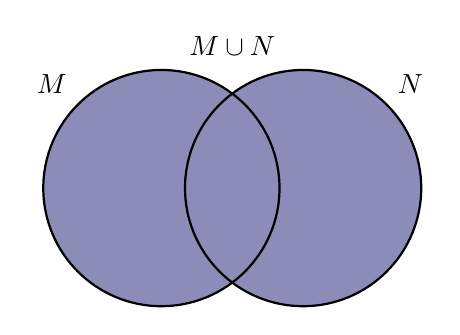
\begin{tikzpicture}[thick,
                set/.style = {circle,
                        minimum size = 3cm,
                        fill=MidnightBlue!50}]
        \node[set,label={135:$M$}] (M) at (0,0) {};
        \node[set,label={45:$N$}] (N) at (1.8,0) {};
        \begin{scope}
                \clip (0,0) circle(1.5cm);
                \clip (1.8,0) circle(1.5cm);
                \fill[MidnightBlue!50](0,0) circle(1.5cm);
        \end{scope}
        \draw (0,0) circle(1.5cm);
        \draw (1.8,0) circle(1.5cm);
        \node at (0.9,1.8) {$M\cup N$};
      \end{tikzpicture}}}$
    }%
    $\vcenter{\hbox{Vereinigungsmenge | Für Mengen M und N: \alert{$M\cup N=\{x: x\in M$ \textbf{oder} $x\in N\}$}}}$
  \end{minipage}
  \onslide<+->
  \begin{minipage}{1\textwidth}
    \centering 
    \scalebox{0.5}{%
      $\vcenter{\hbox{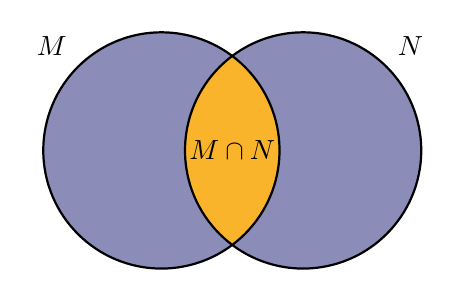
\begin{tikzpicture}[thick,
              set/.style = {circle,
                      minimum size = 3cm,
                      fill=MidnightBlue!50}]
      \node[set,label={135:$M$}] (M) at (0,0) {};
      \node[set,label={45:$N$}] (N) at (1.8,0) {};
      \begin{scope}
              \clip (0,0) circle(1.5cm);
              \clip (1.8,0) circle(1.5cm);
              \fill[Dandelion](0,0) circle(1.5cm);
      \end{scope}
      \draw (0,0) circle(1.5cm);
      \draw (1.8,0) circle(1.5cm);
      \node at (0.9,0) {$M\cap N$};
    \end{tikzpicture}}}$
    }%
    $\vcenter{\hbox{Schnittmenge | Für Mengen M und N: \orongsch{$M\cap N=\{x: x\in M$ \textbf{und} $x\in N\}$}\rule{2.5em}{0em}}}$
  \end{minipage}
  \Halbzeile
  \begin{itemize}[<+->]
    \item Beispiel Vereinigungsmenge
      \begin{itemize}[<+->]
        \item $M=\{\alert<7->{a},\alert<7->{b},\gruen<7->{c}\}$
        \item $N=\{\alert<7->{a},\alert<7->{b},\orongsch<7->{d}\}$
        \item $M\cup N=\{\alert<7->{a},\alert<7->{b},\gruen<7->{c},\orongsch<7->{d}\}$
      \end{itemize}
      \Halbzeile
    \item Beispiel Schnittmenge
      \begin{itemize}[<+->]
        \item $M=\{\gruen<11->{a},\gruen<11->{b},c\}$
        \item $N=\{\gruen<11->{a},\gruen<11->{b}\}$
        \item $M\cap N=\{\gruen<11->{a},\gruen<11->{b}\}$
      \end{itemize}
  \end{itemize}
\end{frame}

\begin{frame}
  {Generalisierte Vereinigungs- und Schnittmenge\only<15>{}}
  \onslide<+->
  \onslide<+->
  \alert{$\bigcup M =\{x: x\in Y$ \textbf{für irgendeine} $Y\in M\}$}\\
  \onslide<+->
  \alert{$\bigcap M =\{x: x\in Y$ \textbf{für jede} $Y\in M\}$}\\
  \Zeile 
  \begin{itemize}[<+->]
    \item Beispiel generalisierte Vereinigungsmenge
      \begin{itemize}[<+->]
        \item $M=\{\{\gruen<7>{a}\},\{\gruen<7>{a},\gruen<8>{b}\},\{\gruen<7>{a},\gruen<8>{b},\gruen<9>{c}\}\}$
        \item $\bigcup M=\{%
            \only<7->{\gruen<7>{a}}%
            \only<8->{,\gruen<8>{b}}%
            \only<9->{,\gruen<9>{c}}%
          \}$
      \end{itemize}
      \Halbzeile
      \onslide<10->
    \item Beispiel generalisierte Schnittmenge
      \begin{itemize}[<+->]
        \item<10-> $M=\{\{\gruen<12>{a}\},\{\gruen<12>{a},\orongsch<13>{b}\},\{\gruen<12>{a},\orongsch<13>{b},\orongsch<14>{c}\}\}$
        \item<11-> $\bigcap M=\{%
            \only<12->{\gruen<12>{a}}
          \}$
      \end{itemize}
  \end{itemize}
\end{frame}

\begin{frame}
  {Differenzmenge und Komplementmenge}
  \onslide<+->
  \onslide<+->
  Differenzmenge | \alert{$M-N=\{x: x\in M$ and $x\not\in N\}$}\\
  \onslide<+->
  Komplementmenge | \alert{$M\backslash N=\{x: x\in N$ and $x\not\in M\}$}\\
  \Halbzeile
  \begin{itemize}[<+->]
    \item Beispiel Differenzmenge
      \begin{itemize}[<+->]
        \item $M=\{\orongsch<7,10>{a},\orongsch<10>{\gruen<7>{b}},\orongsch<10>{\gruen<7>{c}}\}$
        \item $N=\{\orongsch<7>{a}\}$
        \item $M-N=\{\gruen<7>{b},\gruen<7>{c}\}$
      \end{itemize}
      \Halbzeile
    \item Beispiel Komplementmenge
      \begin{itemize}[<+->]
        \item $O=\{\orongsch<10>{a},\orongsch<10>{b},\orongsch<10>{c},\alert<10>{k}\}$
        \item $M\backslash O=\{\alert<10>{k}\}$
      \end{itemize}
      \Halbzeile
    \item Universelles Komplement
      \begin{itemize}[<+->]
        \item die universelle Menge | U=\{x: x is an object\}
        \item $\alert{M^{\prime}}=\{x: x\in U$ and $x\not\in M\}$
      \end{itemize}
  \end{itemize}
\end{frame}

\begin{frame}
  {Triviale Identitäten}
  \onslide<+->
  \onslide<+->
  \centering 
  \begin{tabular}[h]{lccc}
    Idempotenz      & $M\cup M$ & $=$ & $M$ \\
                    & $M\cap M$ & $=$ & $M$ \\
   Kommutativität   & $M\cup N$ & $=$ & $N\cup M$ \\
                    & $M\cap N$ & $=$ & $N\cap M$ \\
   Assoziativität   & $(M\cup N)\cup O$ & $=$ & $M\cup (N\cup O)$ \\
                    & $(M\cap N)\cap O$ & $=$ & $M\cap (N\cap O)$ \\
   Distributivität  & $M\cup (N\cap O)$ & $=$ & $(M\cup N)\cap (M\cup O)$ \\
  \end{tabular}
\end{frame}

\begin{frame}
  {Interessante Identitäten}
  \onslide<+->
  \onslide<+->
  Komplementgesetze\\
  \Halbzeile
  \begin{itemize}[<+->]
    \item $M\cup\emptyset=M$
    \item $M^{\prime\prime}=M$
    \item $M\cap M^{\prime}=\emptyset$
    \item $X\cap U=U$
  \end{itemize}
  \onslide<+->
  \Zeile
  DeMorgan\\
  \Halbzeile
  \begin{itemize}[<+->]
    \item $(M\cup N)^{\prime}=M^{\prime}\cap X^{\prime}$
    \item DeMorgen begegnet uns in der Logik wieder.
  \end{itemize}
\end{frame}

\section{Funktionen und Relationen}

\frame{\frametitle{How to define an ordered pair}
 \begin{itemize}
   \item<1-> \ldots without introducing ordered tuples as a new primitive
   \item<2-> take S=$\{\{a\},\{a,b\}\}$
   \item<3-> we write: \textcolor{blue}{$\langle a,b\rangle = \{\{a\},\{a,b\}\}$}
   \item<4-> orderend n-tuples defined recursively
   \item<5-> $\langle a,b\rangle \not= \langle b,a\rangle$
   \item<6-> first and second coordinate of the tuple
 \end{itemize}
}

\frame{\frametitle{Cartesian products}
 \begin{itemize}
   \item<1-> sets of ordered pairs
   \item<2-> tupling each member of the first argument with each of the second
   \item<3-> \textcolor{blue}{$S_1\times S_2=\{\langle x,y\rangle\|x\in S_1$ and $y\in S_2\}$}
   \item<4-> for an arbitrary number of sets: $S_1\times \cdots \times S_n=\{\langle x_1,x_2,\ldots,x_n\rangle\|x_i\in S_i\} $
   \item<5-> $\langle x_1,x_2,\ldots,x_n\rangle$ abbreviated $\vec{x}$
   \item<6-> for $S\times S\times\cdots$: n-fold products\\ $S^n=\{\vec{s}\|s_i\in S$ for $1\leq i\leq n\}$
 \end{itemize}
}

\frame{\frametitle{Defintion of relations}
 \begin{itemize}
   \item<1-> hold between (sets of) objects
   \item<2-> \emph{x kicks y}, \emph{x lives on the same floor as y}, \ldots
   \item<3-> formalization: \textcolor{blue}{Rab}, \textcolor{blue}{aRb}
   \item<4-> \textcolor{blue}{$a\in A$ and $b\in B$: $R \subseteq A\times B$,\\ R is from A
 (\textbf{domain}) to B (\textbf{range})}
   \item<5-> R from A to A is \textcolor{blue}{in A}
 \end{itemize}
}

\frame{\frametitle{Complement, inverse}
 \begin{itemize}
   \item<1-> complement \textcolor{blue}{$R^{\prime}=\{\langle a,b\rangle\ \not\in R\}$ for $R\subseteq A\times B$}
      \begin{itemize}
        \item<2-> R = the relation of teacherhood between a and b (the \textbf{arguments})
        \item<3-> R$^{\prime}$ = all pairs $\langle b,a\rangle$ s.t. it is false that the first member is the teacher of the second member
      \end{itemize}
   \item<4-> inverse: \textcolor{blue}{$R^{-1}=\{\langle b,a\rangle\|\langle a,b\rangle\in R\}$  for $R\subseteq A\times B$}
      \begin{itemize}
        \item<5-> R = the relation of teacherhood between a and b:\\ \emph{Herr Webelhuth is the teacher of Herr Sch\"afer.}
        \item<6-> R$^{-1}$ = all pairs $\langle b,a\rangle$ where $a$ is the teacher of $b$:\\ \emph{Herr Sch\"afer is the inverse-teacher of Herr Webelhuth.}
      \end{itemize}  
 \end{itemize}
}
\frame{\frametitle{Functions}
\begin{itemize}
  \item<1-> \textcolor{blue}{A function F from A to B is a relation s.t. for every $a\in A$ there is exactly on tuple $\langle a,b\rangle\in A\times B$ s.t. $a$ is the first coordinate.}
  \item<2-> partial function from A to B: for some $a\in A$ there is no tuple $\langle a,b\rangle\in A\times B$,  F is not \emph{defined for} some $a$ 
\end{itemize}
}

\frame{\frametitle{Injection, surjection, bijection}
\begin{itemize}
  \item<1-> B the range of F, F is \textbf{into} B
  \item<2-> F from A to B is \textcolor{blue}{\textbf{onto (a \textbf{surjection})} B iff there is no $b_i\in B$ s.t. there is no $\langle a,b_i\rangle\in F$}
  \item<3-> F from A to B is \textcolor{blue}{\textbf{one-to-one (an \textbf{injection})} iff there are no two pairs s.t. $\langle a_i,b_j\rangle\in F$ and $\langle a_k,b_j\rangle\in F$}
  \item<4-> one-to-one, onto, and total function: correspondence (bijection)
\end{itemize}
}

\frame{\frametitle{Composition}
\begin{itemize}
  \item<1-> One can take the range of a function and make it the domain of another function.
  \item<2-> \textcolor{blue}{A function $F_1:A\rightarrow B$ and a function $F_2:B\rightarrow C$ can be composed as $B(A(a))$, short $B\circ A$}
  \item<3-> the compound function can be empty, it will be total if both A and B are bijections.
\end{itemize}
}

\section{Mehr über Relationen und Mengen}


\frame{\frametitle{Reflexivity}
A relation R in $A=\{a,b,\ldots\}$ is...\\

\bigskip
{\small
\begin{tabular}{ll|l}
  & if & (ex.) \\
  \hline
  reflexive & for \textbf{every $a\in A$}: $\langle a,a\rangle\in R$ & is as heavy as\\
       & & {\scriptsize A: physical objects} \\
  irreflexive & for \textbf{every $a\in A$}: $\langle a,a\rangle\not\in R$ & is the father of \\
  non-reflexive & for \textbf{some $a\in A$}: $\langle a,a\rangle\not\in R$ & has hurt \\
\end{tabular}}
}

\frame{\frametitle{Symmetry}
A relation R in $A=\{a,b,\ldots\}$ is...\\

\bigskip
{\small
\begin{tabular}{ll|l}
  & if & (ex.) \\
  \hline
  symmetric & for every $\langle a,b\rangle\in R$: & has the same car as\\
            & $\langle b,a\rangle\in R$ & \\
  asymmetric & for every $\langle a,b\rangle\in R$: & has a different car than \\
             & $\langle b,a\rangle\not\in R$ & \\
  non-symmetric & for some $\langle a,b\rangle\in R$: & is the sister of \\
               & $\langle b,a\rangle\not\in R$ & \\
	       anti-symmetric &  for every $\langle a,b\rangle\in R$: $a=b$ & beats oneself\\
                  &                               & {\scriptsize not every human does}\\
\end{tabular}}
}

\frame{\frametitle{Transitivity}
A relation R in $A=\{a,b,\ldots\}$ is...\\

\bigskip
{\small
\begin{tabular}{ll|l}
  & if & (ex.) \\
  \hline
  transitive & if $\langle a,b\rangle\in R$ and $\langle b,c\rangle\in R$ & is to the left of\\
            & then $\langle a,c\rangle\in R$ &  \\
  intransitive & the above is never the case & is the father of \\
  non-transitive & the above is sometimes not the case & likes \\
\end{tabular}}
}

\frame{\frametitle{Connectedness}
A relation  R in $A=\{a,b,\ldots\}$ is...\\

\bigskip
{\small
\begin{tabular}{ll|l}
  & if & (ex.) \\
  \hline
  connected & for every $a,b\in A$, $a\not =b$: & $>$ \\
            & either $\langle a,b\rangle\in R$ or $\langle b,a\rangle\in R$ & {\scriptsize (A: the natural numbers)} \\
  non-connected & for some $a,b\in A$  & likes \\
                & the above is not the case & \\
\end{tabular}}
}

\frame{\frametitle{Equivalence relations}
\begin{itemize}
  \item<1-> reflexive \footnotesize{($\langle a,a\rangle\in R$ for every $a$)}
  \item<2-> symmetric \footnotesize{($\langle b,a\rangle\in R$ for every $\langle a,b\rangle$)}
  \item<3-> transitive \footnotesize{($\langle a,b\rangle\in R$ \& $\langle b,c\rangle\in R\rightarrow\langle a,c\rangle\in R$)}
  \item<4-> \emph{is as stupid as}
  \item<5-> partition the range into equivalence classes:\\$A=\{a,b,c,d\}$, for example $P_{A_1}=\{\{a,b\},\{c\},\{d\}\}$
  \item<6-> \textcolor{red}{not} $\{\{a\},\{b,c\}\}$ or $\{\{a,b\},\{b,c\},\{d\}\}$
\end{itemize}  
}

\frame{\frametitle{Defining ordering relations}
An ordering relation R in A is ...
\begin{itemize}
  \item<1-> transitive \footnotesize{($\langle a,b\rangle\in R$ \& $\langle b,c\rangle\in R\rightarrow\langle a,c\rangle\in R$)} \ldots plus \ldots
  \item<2-> \textcolor{blue}{irreflexive and asymmetric: \textbf{strict order}}
  \item<3-> {\footnotesize $A=\{a,b,c,d\}$, $R_1=\{\langle a,b\rangle, \langle b,c\rangle, \langle a,c\rangle\}$}
  \item<4-> \textcolor{blue}{reflexive and anti-symmetric: \textbf{weak order}}
  \item<5-> {\footnotesize $A=\{a,b,c,d\}$, $R_1=\{\langle a,a\rangle, \langle b,b\rangle, \langle c,c\rangle, \langle a,b\rangle, \langle b,c\rangle, \langle a,c\rangle \}$}  
\end{itemize}
}

\frame{\frametitle{Orders: an example}
\begin{itemize}
  \item<1-> a strict order: \emph{greater than} ($>$) in $\mathbb{N}$
  \item<2-> what is the corresponding weak order
  \item<3-> $\geq$
\end{itemize}
}

\frame{\frametitle{}
\begin{itemize}
  \item<1-> \textbf{minimal}: x is not preceded
  \item<2-> \textbf{least}: x precedes every other lement
  \item<3-> \textbf{maximal}: x is not succeeded
  \item<4-> \textbf{greatest}: x succeeds every other element
  \item<5-> \textbf{well-ordering}: total order, every subset has a least element
\end{itemize}
}

% \section{Mächtigkeiten}
% 
% 
% \frame{\frametitle{The number of elements\ldots}
% \begin{itemize}
%   \item<1-> $A=\{a,b,c\}$
%   \item<2-> $B=\{a,b,c\}$
%   \item<3-> obviously, $A=B$ (equal)
%   \item<4-> there is an $R$ from A to B s.t. $R=\{\langle a,a\rangle,\langle b,b\rangle,\langle c,c\rangle\}$
%   \item<5-> for every set C with the same number of elements\\ (e.g., $C=\{1,2,3\}$): 
%          $R=\{\langle a,1\rangle,\langle b,2\rangle,\langle c,3\rangle\}$
%   \item<6-> such relations are one-to-one correspondences
% \end{itemize}
% }
% 
% \frame{\frametitle{Denumerable sets}
% \begin{itemize}
%   \item<1-> $\mathbb{N}$ is infinite
%   \item<2-> for every A there is some R\Sub{card}
%        \begin{itemize}
%          \item<3-> a one-to-one correspondence
%          \item<4-> from A's members to the first $n$ members of $\mathbb{N}$
%          \item<5-> s.t. $n$ is the \textcolor{blue}{cardinality of A, $\|A\|$}
%       \end{itemize}
%   \item<6-> sets A,B with $\|A\|=\|B\|$ are \textcolor{blue}{equivalent}
%   \item<7-> $\|\mathbb{N}\|=\aleph^0$
% \end{itemize}
% }
% 
% 
% \frame{\frametitle{A problem}
% \begin{itemize}
%   \item<1-> \textcolor{red}{for some sets there is no such R\Sub{card}}
%   \item<2-> no way of bringing their elements into an exhaustive linear order
%   \item<3-> no problem with $\mathbb{Q}$: 
%     \begin{small}\Treek[2]{2}{
% 	    & \K{$\ra{0,1}$}\ARkk{0,0}{0,0}{dl} & \K{$\ra{0,2}$}\ARkk{0,0}{0,0}{dl}\ARr{dll} & \K{$\ra{0,3}$}\ARkk{0,0}{3,0}{dl}\ARr{ddlll} & \K{$\cdots$}\ARkk{0,0}{0,0}{dl}\\
% 	    \K{$\ra{1,0}$} & \K{$\ra{1,1}$}\ARkk{-3,0}{0,0}{dl}        & \K{$\ra{1,2}$}\ARkk{0,0}{0,0}{dl} & \K{$\ra{1,3}$}\ARkk{0,0}{0,0}{dl} & \K{$\cdots$}\ARkk{0,0}{0,0}{dl} \\
% 	    \K{$\ra{2,0}$} & \K{$\ra{2,1}$}\ARkk{0,0}{0,0}{dl}        & \K{$\ra{2,2}$}\ARkk{0,0}{0,0}{dl} & \K{$\ra{2,3}$}\ARkk{0,0}{0,0}{dl} & \K{$\cdots$}\ARkk{0,0}{0,0}{dl} \\
%     \K{$\vdots$}   & \K{$\vdots$}          & \K{$\vdots$}   & \K{$\vdots$}   &  \\
%     }\end{small}
% \end{itemize}
% }
% 
% \frame{\frametitle{The non-denumerable real numbers}
% \begin{itemize}
%   \item<1-> now: $\mathbb{R}$
%   \item<2-> some elements cannot be represented as an ordered pair of two elements of $\mathbb{N}$
%   \item<3-> in $[0,1]$, every real can be represented as \textcolor{blue}{$0.abcdefg\ldots$}, $a,b,c,d,e,f,g,\ldots\in\{0,1,2,3,4,5,6,7,8,9\}$
% \end{itemize}
% }
% 
% \frame{\frametitle{Trying to enumerate}
% \begin{itemize}
%   \item<1-> an enumeration of $[0,1]$ in $\mathbb{R}$?\\
%   
%   \medskip
%   \begin{tabular}{ccccccccc}
%      x\Sub{1} & = & 0 & . & a\Sub{11} & a\Sub{12} & a\Sub{13} & a\Sub{14} & \ldots \\
%      x\Sub{2} & = & 0 & . & a\Sub{21} & a\Sub{22} & a\Sub{23} & a\Sub{24} & \ldots \\
%      x\Sub{3} & = & 0 & . & a\Sub{31} & a\Sub{32} & a\Sub{33} & a\Sub{34} & \ldots \\
%       $\vdots$ & & \vdots &&&&& \\     
%      x\Sub{n} & = & 0 & . & a\Sub{n1} & a\Sub{n2} & a\Sub{n3} & a\Sub{n4} & \ldots \\
%   \end{tabular}
% \end{itemize}
% }
% 
% \frame{\frametitle{Failing to enumerate}
% \begin{itemize}
%   \item<1-> What about an $x_m$ which differs from $x_n$ at $a_{nn}$\\
%   
%   \medskip
%   {\footnotesize\begin{center}\begin{tabular}{ccccccccc}
%      x\Sub{1} & = & 0 & . & \textcolor{red}{a\Sub{11}} & a\Sub{12} & a\Sub{13} & a\Sub{14} & \ldots \\
%      x\Sub{2} & = & 0 & . & a\Sub{21} & \textcolor{red}{a\Sub{22}} & a\Sub{23} & a\Sub{24} & \ldots \\
%      x\Sub{3} & = & 0 & . & a\Sub{31} & a\Sub{32} & \textcolor{red}{a\Sub{33}} & a\Sub{34} & \ldots \\
%       $\vdots$ & & \vdots &&&&& \\     
%      x\Sub{n} & = & 0 & . & a\Sub{n1} & a\Sub{n2} & a\Sub{n3} & \textcolor{red}{a\Sub{nn}} & \ldots \\
%   \end{tabular}\end{center}}
%   
%   \item<2-> \textcolor{red}{It won't be in the array...}
%   \item<3-> $\mathbb{R}$ is non-denumerable
%   \item<4-> If $\|A\|=\aleph^0$ then $\|\wp(A)\|=2^{\aleph_0}$ (cf. Partee et al. 62f.)
% \end{itemize}
% }
